% Copyright 2004 by Till Tantau <tantau@users.sourceforge.net>.
%
% In principle, this file can be redistributed and/or modified under
% the terms of the GNU Public License, version 2.
%
% However, this file is supposed to be a template to be modified
% for your own needs. For this reason, if you use this file as a
% template and not specifically distribute it as part of a another
% package/program, I grant the extra permission to freely copy and
% modify this file as you see fit and even to delete this copyright
% notice. 

\documentclass{beamer}

% There are many different themes available for Beamer. A comprehensive
% list with examples is given here:
% http://deic.uab.es/~iblanes/beamer_gallery/index_by_theme.html
% You can uncomment the themes below if you would like to use a different
% one:
%\usetheme{AnnArbor}
%\usetheme{Antibes}
%\usetheme{Bergen}
%\usetheme{Berkeley}
%\usetheme{Berlin}
%\usetheme{Boadilla}
%\usetheme{boxes}
%\usetheme{CambridgeUS}
%\usetheme{Copenhagen}
%\usetheme{Darmstadt}
%\usetheme{default}
%\usetheme{Frankfurt}
%\usetheme{Goettingen}
%\usetheme{Hannover}
%\usetheme{Ilmenau}
%\usetheme{JuanLesPins}
%\usetheme{Luebeck}
%\usetheme{Madrid}
%\usetheme{Malmoe}
%\usetheme{Marburg}
%\usetheme{Montpellier}
%\usetheme{PaloAlto}
%\usetheme{Pittsburgh}
%\usetheme{Rochester}
%\usetheme{Singapore}
%\usetheme{Szeged}
%\usetheme{Warsaw}

\usepackage{amsmath}
\usepackage{textpos}
\usepackage{ulem}

\definecolor{BYUblue}{RGB}{0,31,69}
\definecolor{BYUgold}{RGB}{195,163,106}
\usecolortheme[RGB={0,31,69}]{structure} % BYU Blue

\definecolor{metric-PR}{RGB}{200,127,0}
\definecolor{metric-NE}{RGB}{51,51,255}
\definecolor{metric-OFI}{RGB}{204,0,0}
\definecolor{metric-IRO}{RGB}{0,102,51}

\usetheme{Frankfurt}
\setbeamercolor*{section in head/foot}{bg=BYUblue,fg=gray!25}
\setbeamercolor*{frametitle}{bg=BYUblue!50,fg=white!25}
\setbeamercovered{transparent}
\mode<all>

\DeclareMathOperator*{\argmax}{arg\,max}

\title{Submodular optimization}

%\subtitle{Optional Subtitle}

\author{ Daqing Yi }


\institute
{
  HCMI lab\\
  Brigham Young University
}

\date[]{} 

\addtobeamertemplate{frametitle}{}{%
\begin{textblock*}{100mm}(0.9\textwidth,-1.2cm)

\includegraphics[width=1.1cm]{figure/BYU_logo.png}
\end{textblock*}}

\begin{document}

\begin{frame}
  \titlepage
\end{frame}

\begin{frame}{Outline}{Structure}
  \tableofcontents
  % You might wish to add the option [pausesections]
\end{frame}

\section{Introduction}

\begin{frame}{Modeling human intent}{Path Planning}
THe problem in modeling human intent
\begin{itemize}
\item incomparability in objectives
\item conflict in objectives
\item hardness in weighing the objectives
\item vagueness in importance selection
\end{itemize}
\begin{figure}
\centering
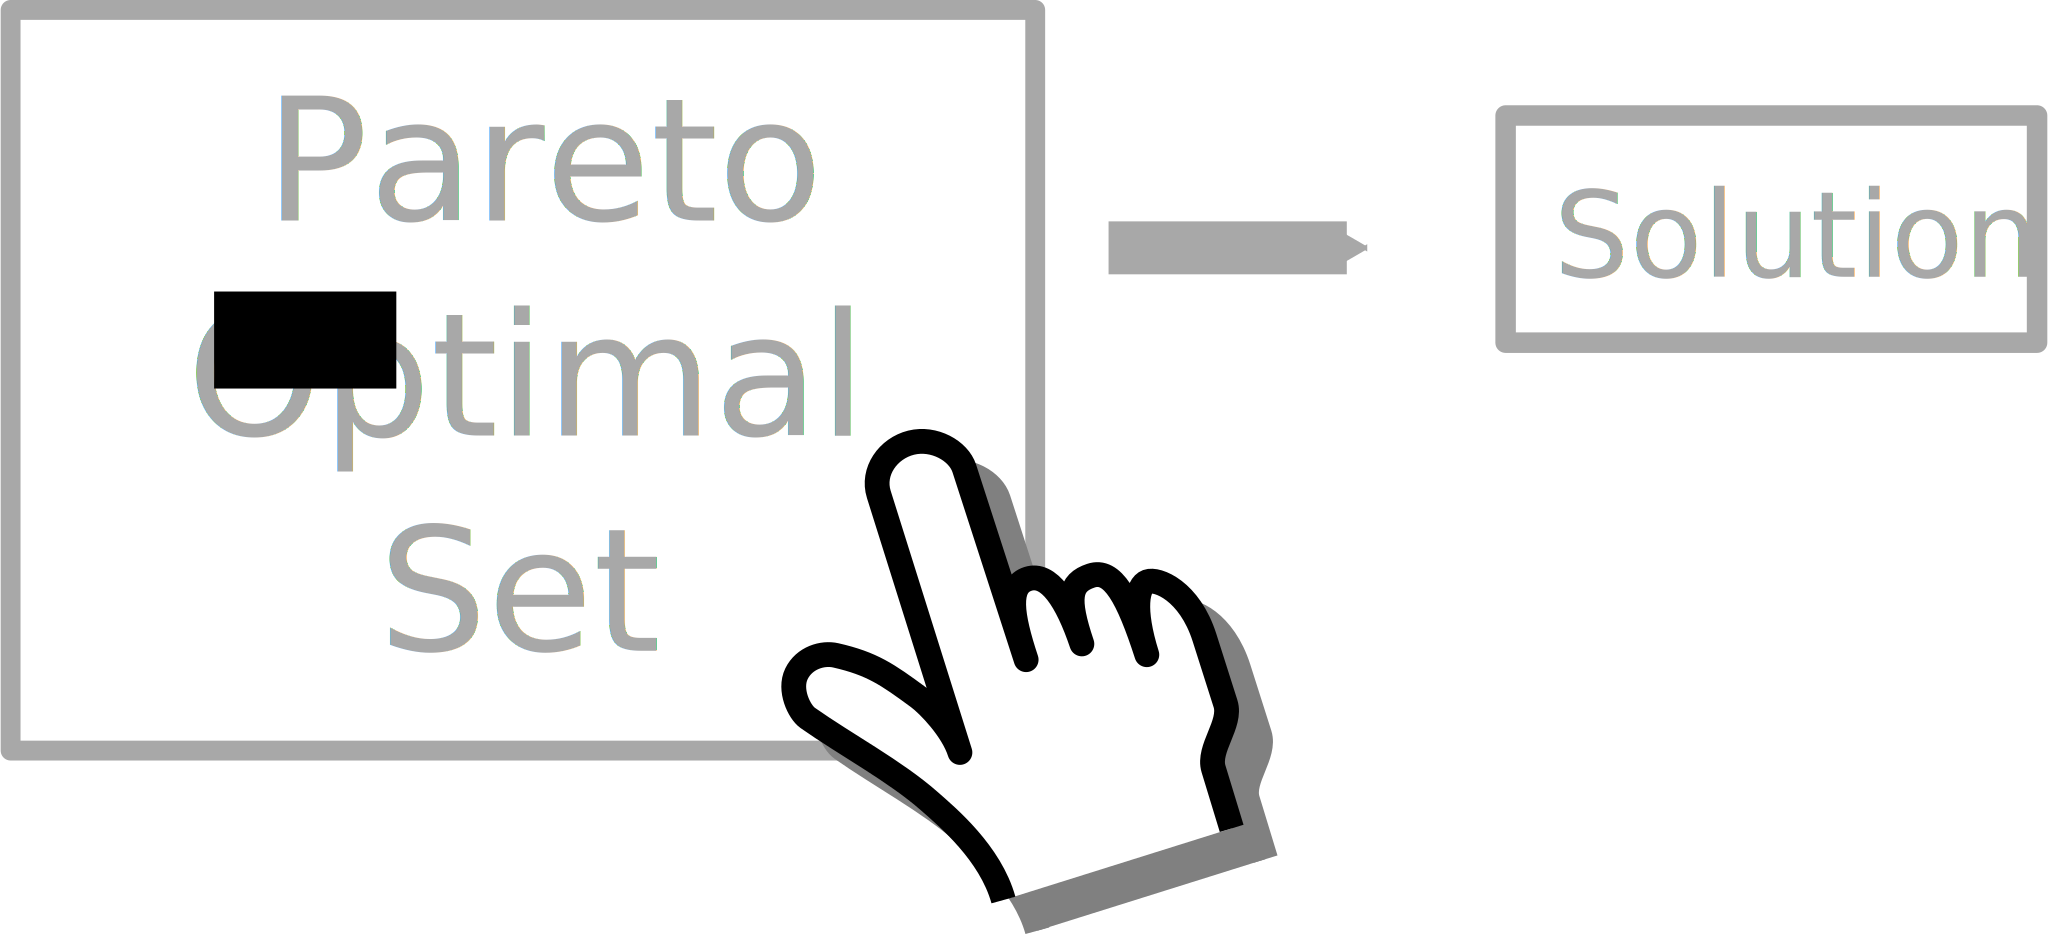
\includegraphics[width=0.6\linewidth]{figure/human_interactive_moo}
%\caption{}
\label{fig:human_interactive_moo}
\end{figure}
\end{frame}

\begin{frame}{Pareto Optimal}{}
\end{frame}

\section{Submodular}

\begin{frame}{Submodular}{Submodular}
\begin{frame}
	\begin{block}{}
		\begin{equation}
		\nonumber
		f(x_{1} , \cdots , x_{N} )= f(x_{1}) + \cdots + f(x_{N})
		\end{equation}
	\end{block}
\end{frame}
\end{frame}

\begin{frame}{Sensor placement}{Maximum coverage}
	
\end{frame}

\begin{frame}{Sensor placement}{MAP inference}
	
\end{frame}


\section{Path Planning}

\begin{frame}{Informative Path Planning}{Information measurement}
\begin{itemize}
\item minimize the uncertainty of the observed environment
\end{itemize}
\begin{figure}
	\centering
	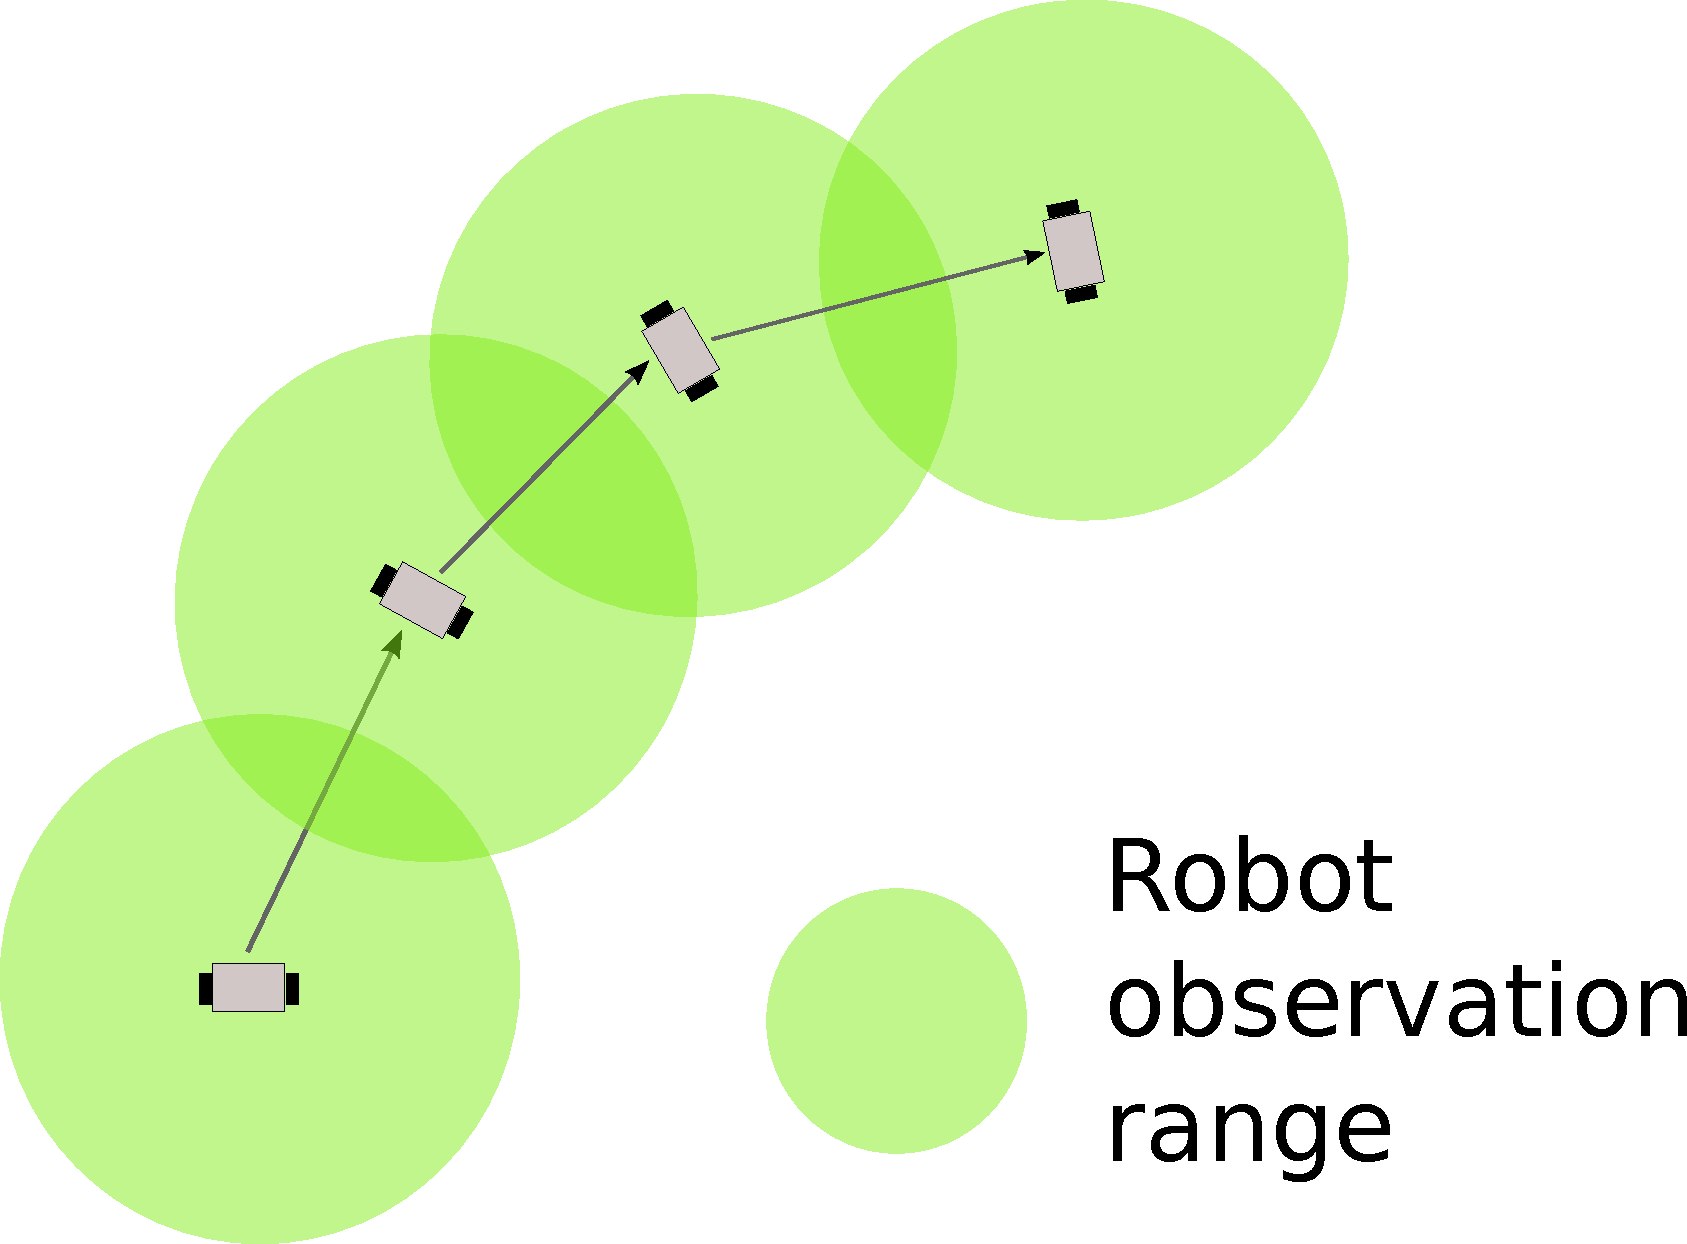
\includegraphics[width = .6\textwidth]{./figure/robotObservation}
\end{figure}
\end{frame}

\begin{frame}{Cordon and search}{Application}
\begin{columns}
	\column{0.5\textwidth}
	\begin{minipage}{\textwidth}
		\begin{figure}
			\centering
			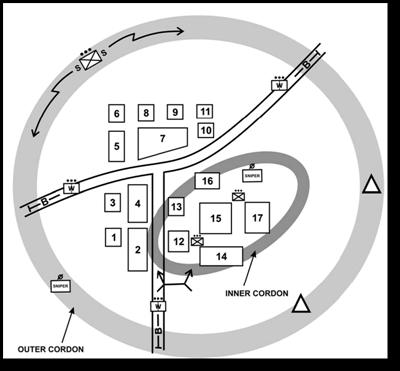
\includegraphics[width = 0.9\textwidth]{./figure/cordon_and_search.jpg}
		\end{figure}
	\end{minipage}
	
	\column{0.5\textwidth}
	\begin{minipage}{\textwidth}
		\begin{figure}
			\centering
			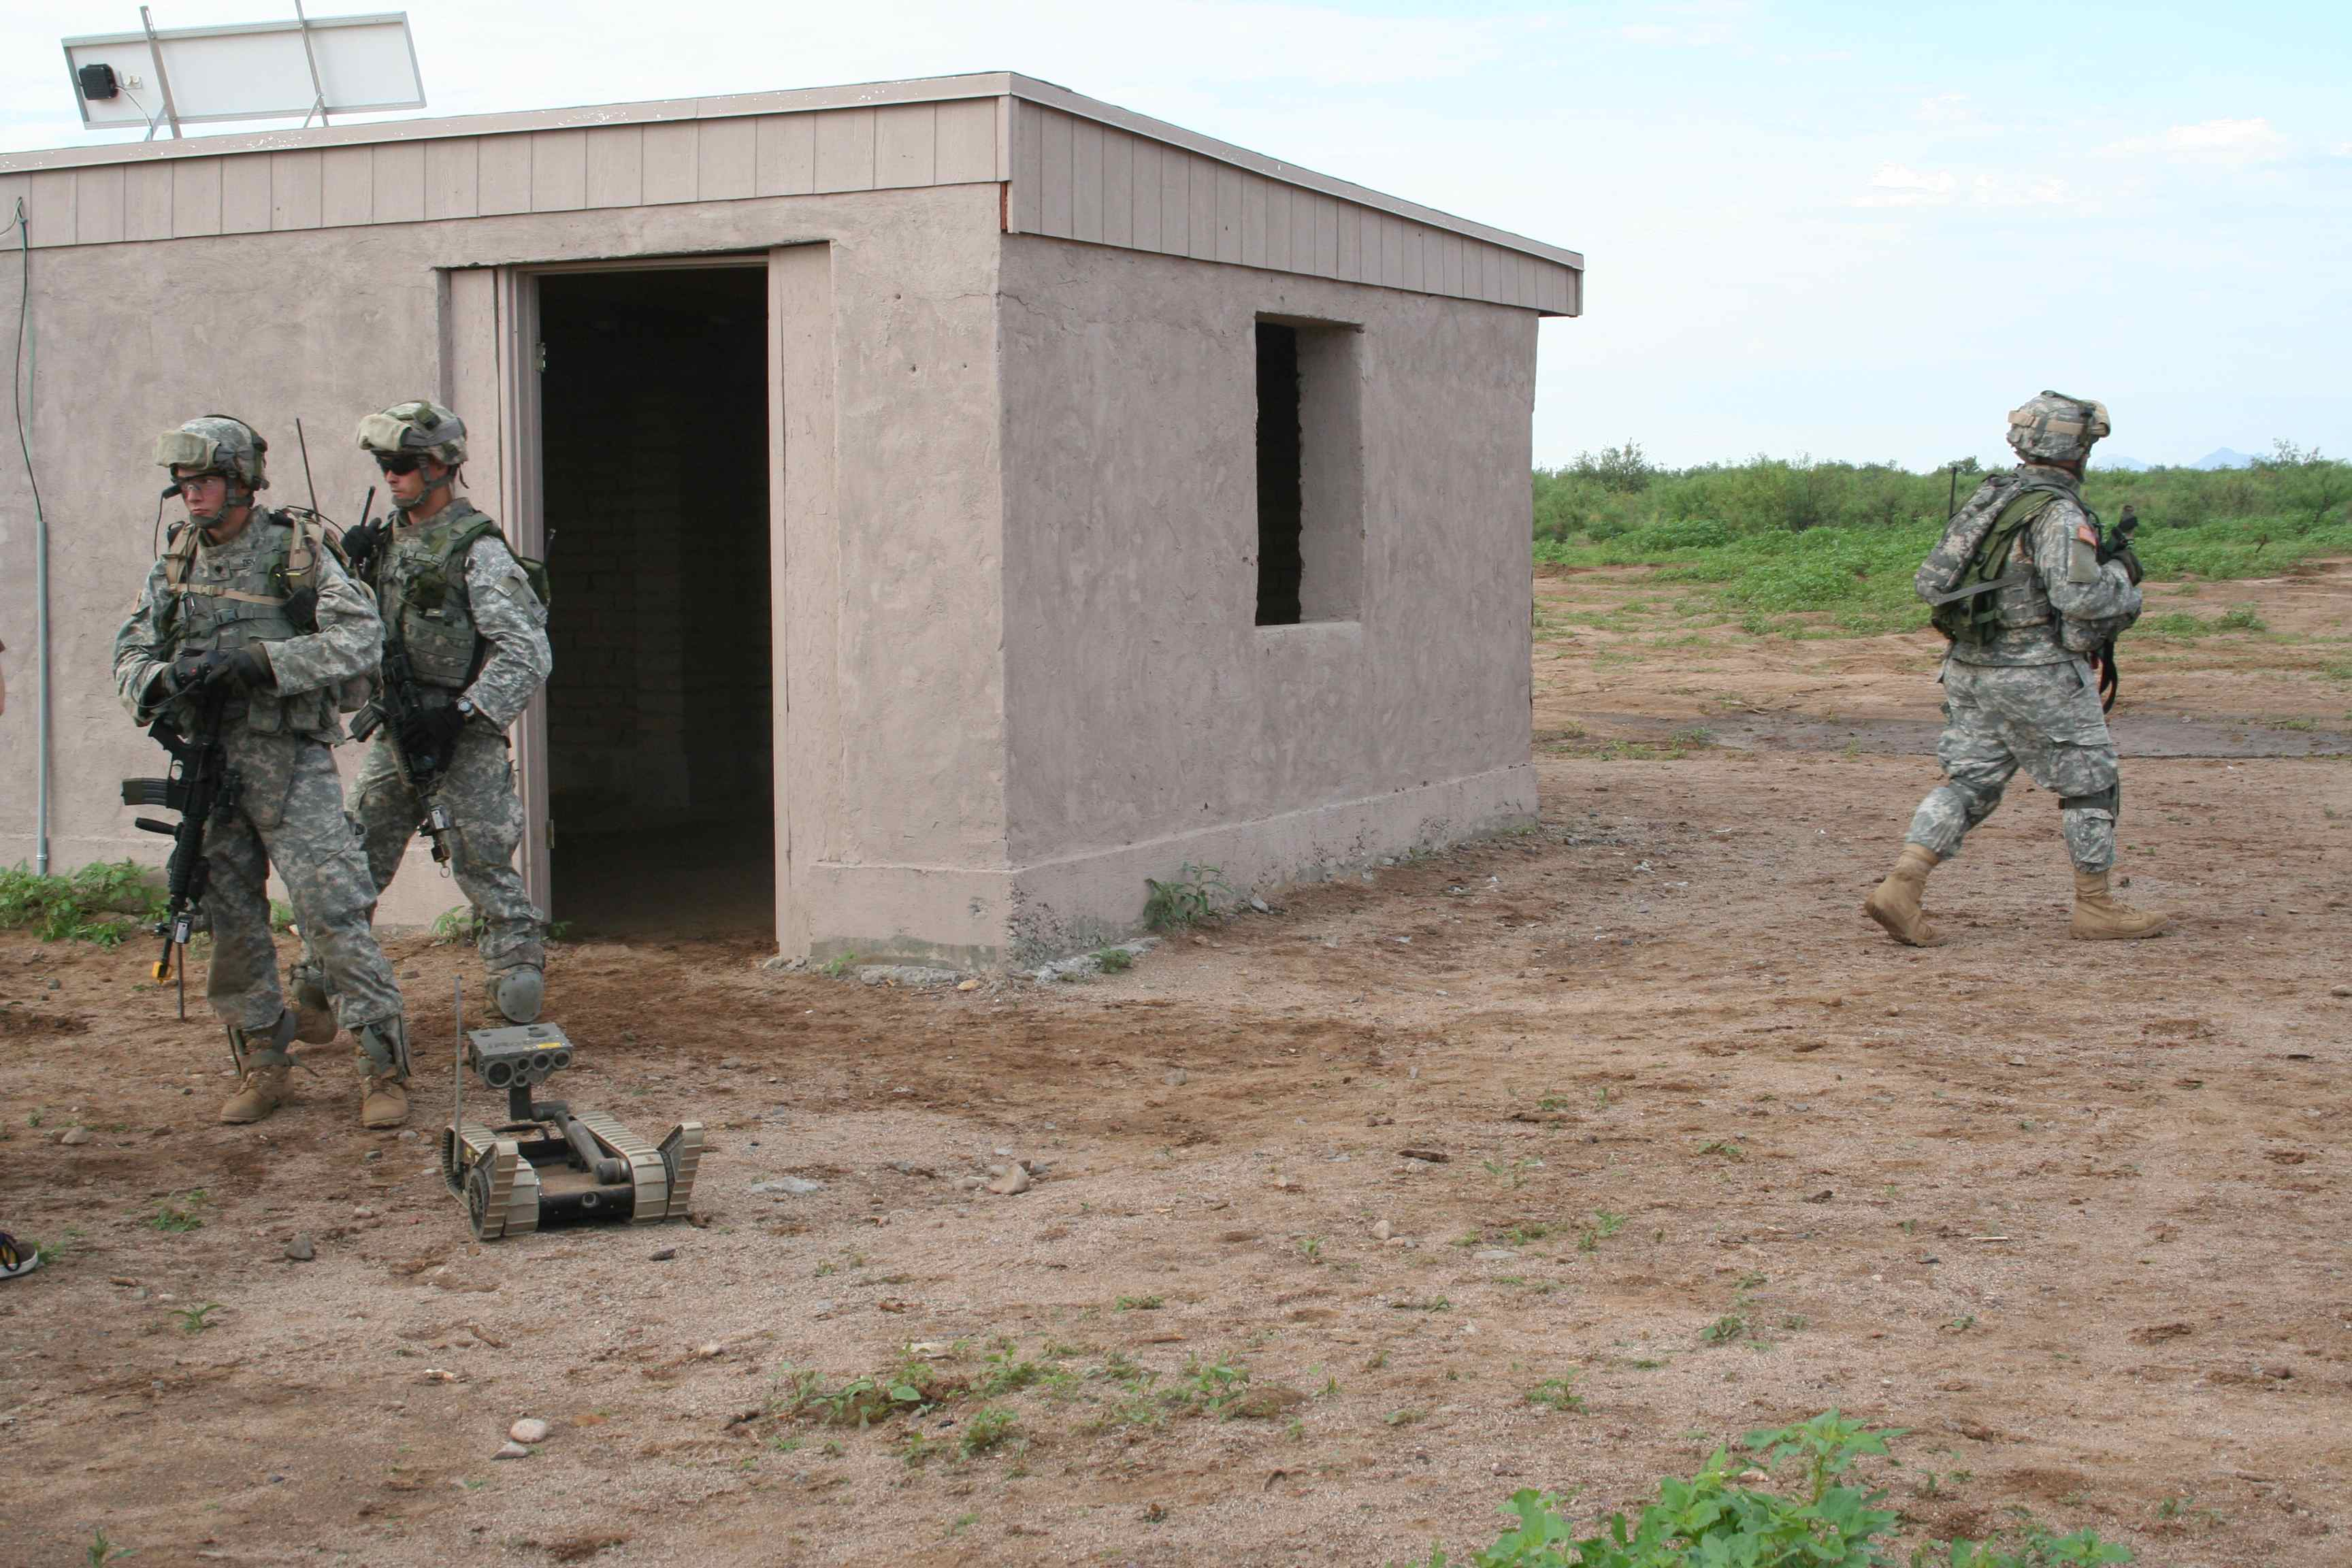
\includegraphics[width = 0.9\textwidth]{./figure/soldier_and_robot.jpg}
		\end{figure}
	\end{minipage}	
\end{columns}
\end{frame}

\begin{frame}{Map discretization}{Application}
	\begin{columns}
		\column{0.5\textwidth}
		\begin{minipage}{\textwidth}
			\begin{figure}
				\centering
				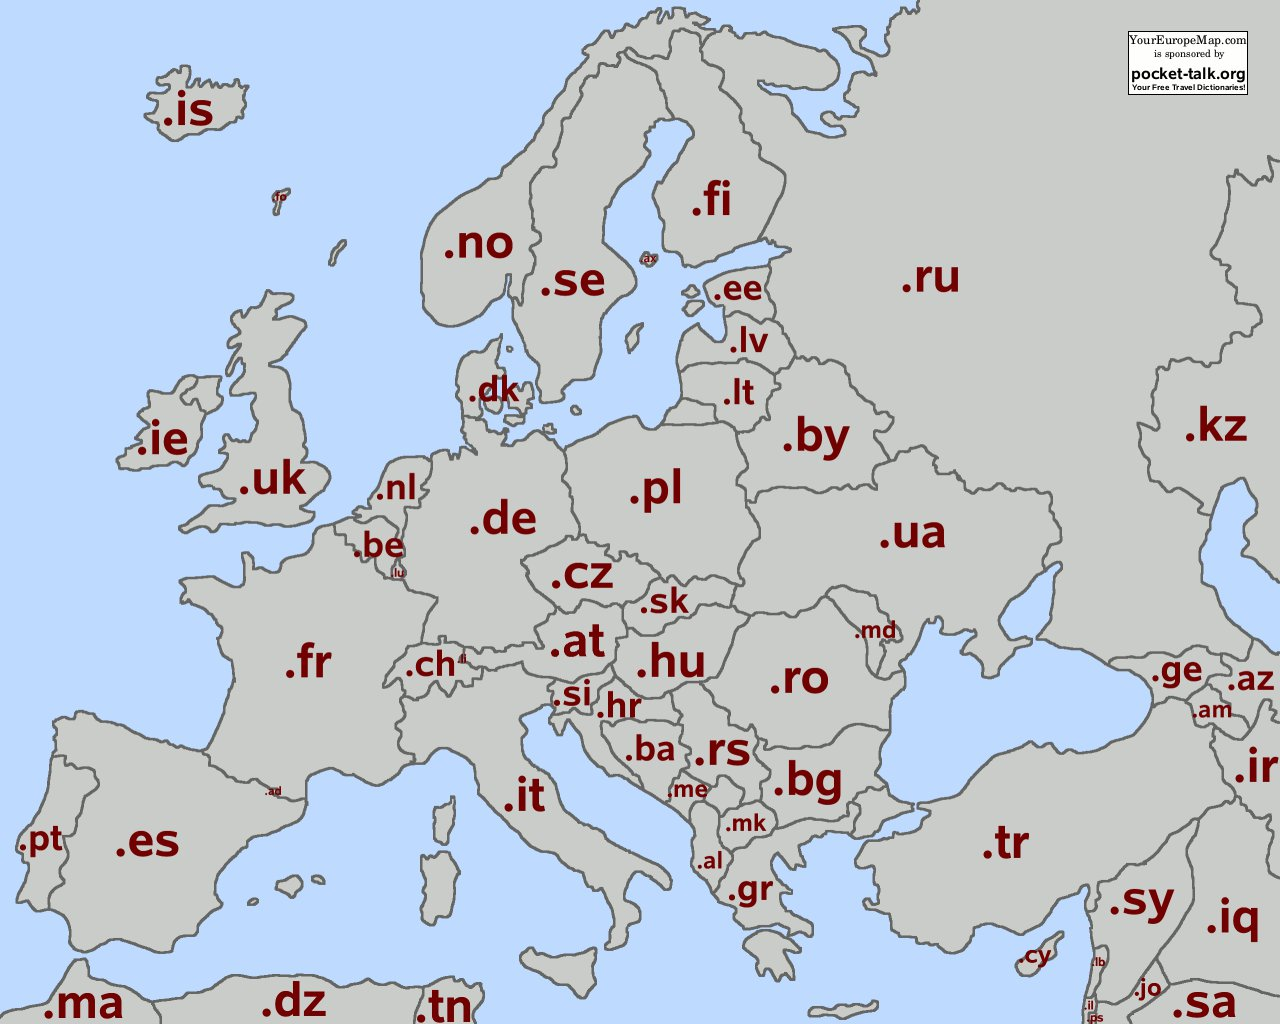
\includegraphics[width = 0.9\textwidth]{./figure/map_tld_europe.jpg}
			\end{figure}
		\end{minipage}
		
		\column{0.5\textwidth}
		\begin{minipage}{\textwidth}
			\begin{figure}
				\centering
				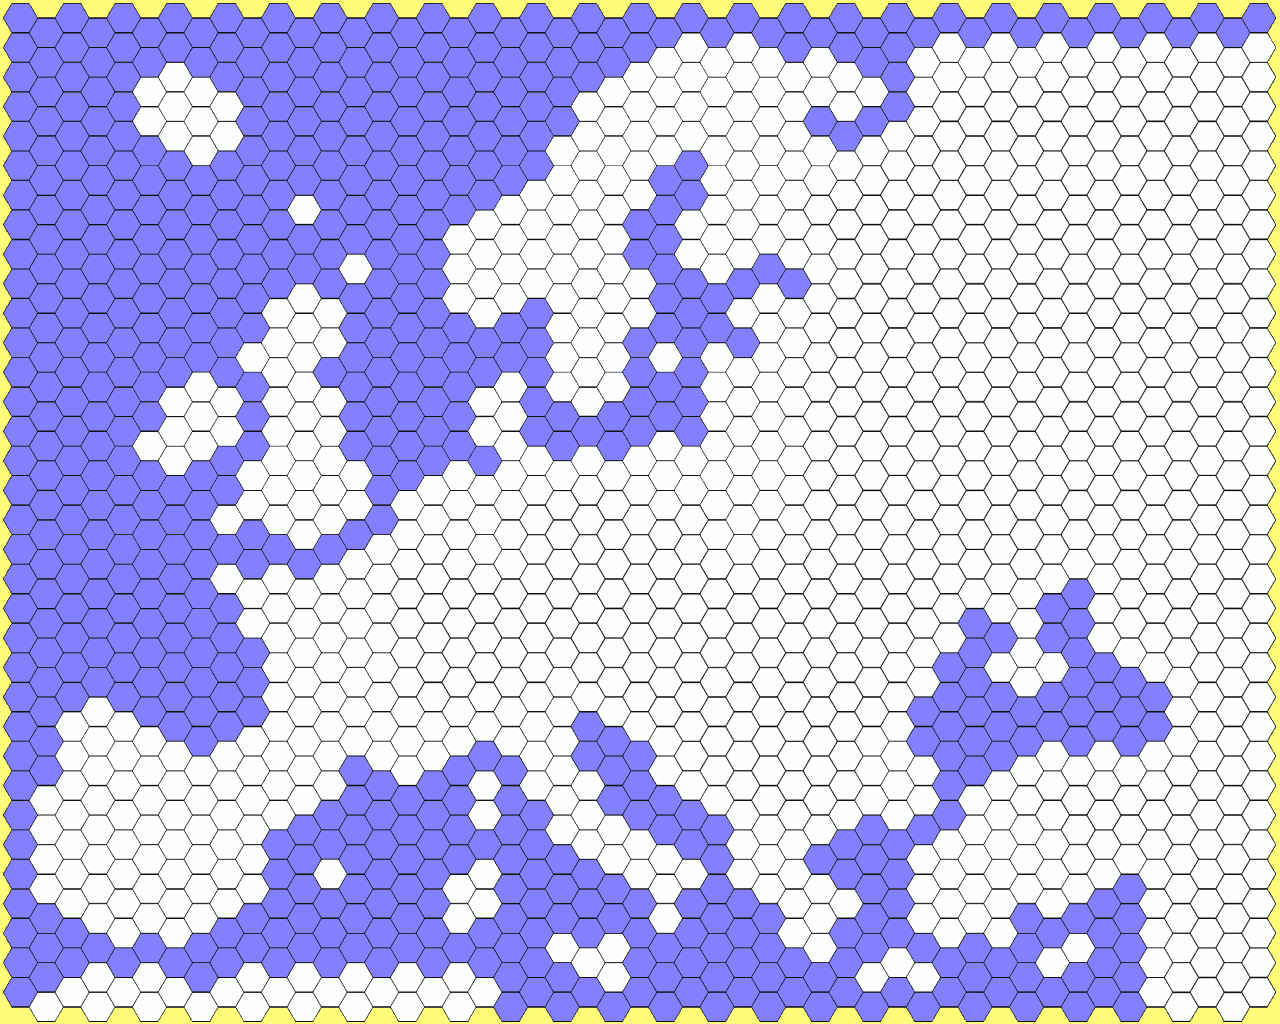
\includegraphics[width = 0.9\textwidth]{./figure/hexagonal_europe_map.png}
			\end{figure}
		\end{minipage}	
	\end{columns}
\end{frame}

\begin{frame}{Submodular orienteering}{Informative path}
	\begin{itemize}
	\item $ \mathbf{S} $ - Environment states
	\item $ \mathbf{O}^{X} $ - Robot's observations
	\item $ \mathbf{O}^{Y^{h}} $ - Human's obeservations
	\end{itemize}
	\begin{block}{Conditional mutual information}
		$ I(\mathbf{S}; \mathbf{O}^{X} \mid \mathbf{O}^{Y^{h}}) = H(\mathbf{S} \mid \mathbf{O}^{Y^{h}}) - H(\mathbf{S} \mid \mathbf{O}^{X},\mathbf{O}^{Y^{h}}) $
	\end{block} 
	
	\bigskip
	
	\begin{itemize}
		\item Entropy reduction
		\item Submodularity
		\item Chain rule \\
		$ I(\mathbf{S}; \mathbf{O}^{X} \mid \mathbf{O}^{Y^{h}}) = \sum_{t=1}^{T} I(O^{X}_{t} ; \mathbf{S} \mid O^{X}_{1} , \cdots , O^{X}_{t-1}, \mathbf{O}^{Y^{h}}) $
	\end{itemize}
	
\end{frame}

%\subsection{Human constraint}

\begin{frame}{Team role}{Human constraint}
	
	\begin{figure}
		\centering
		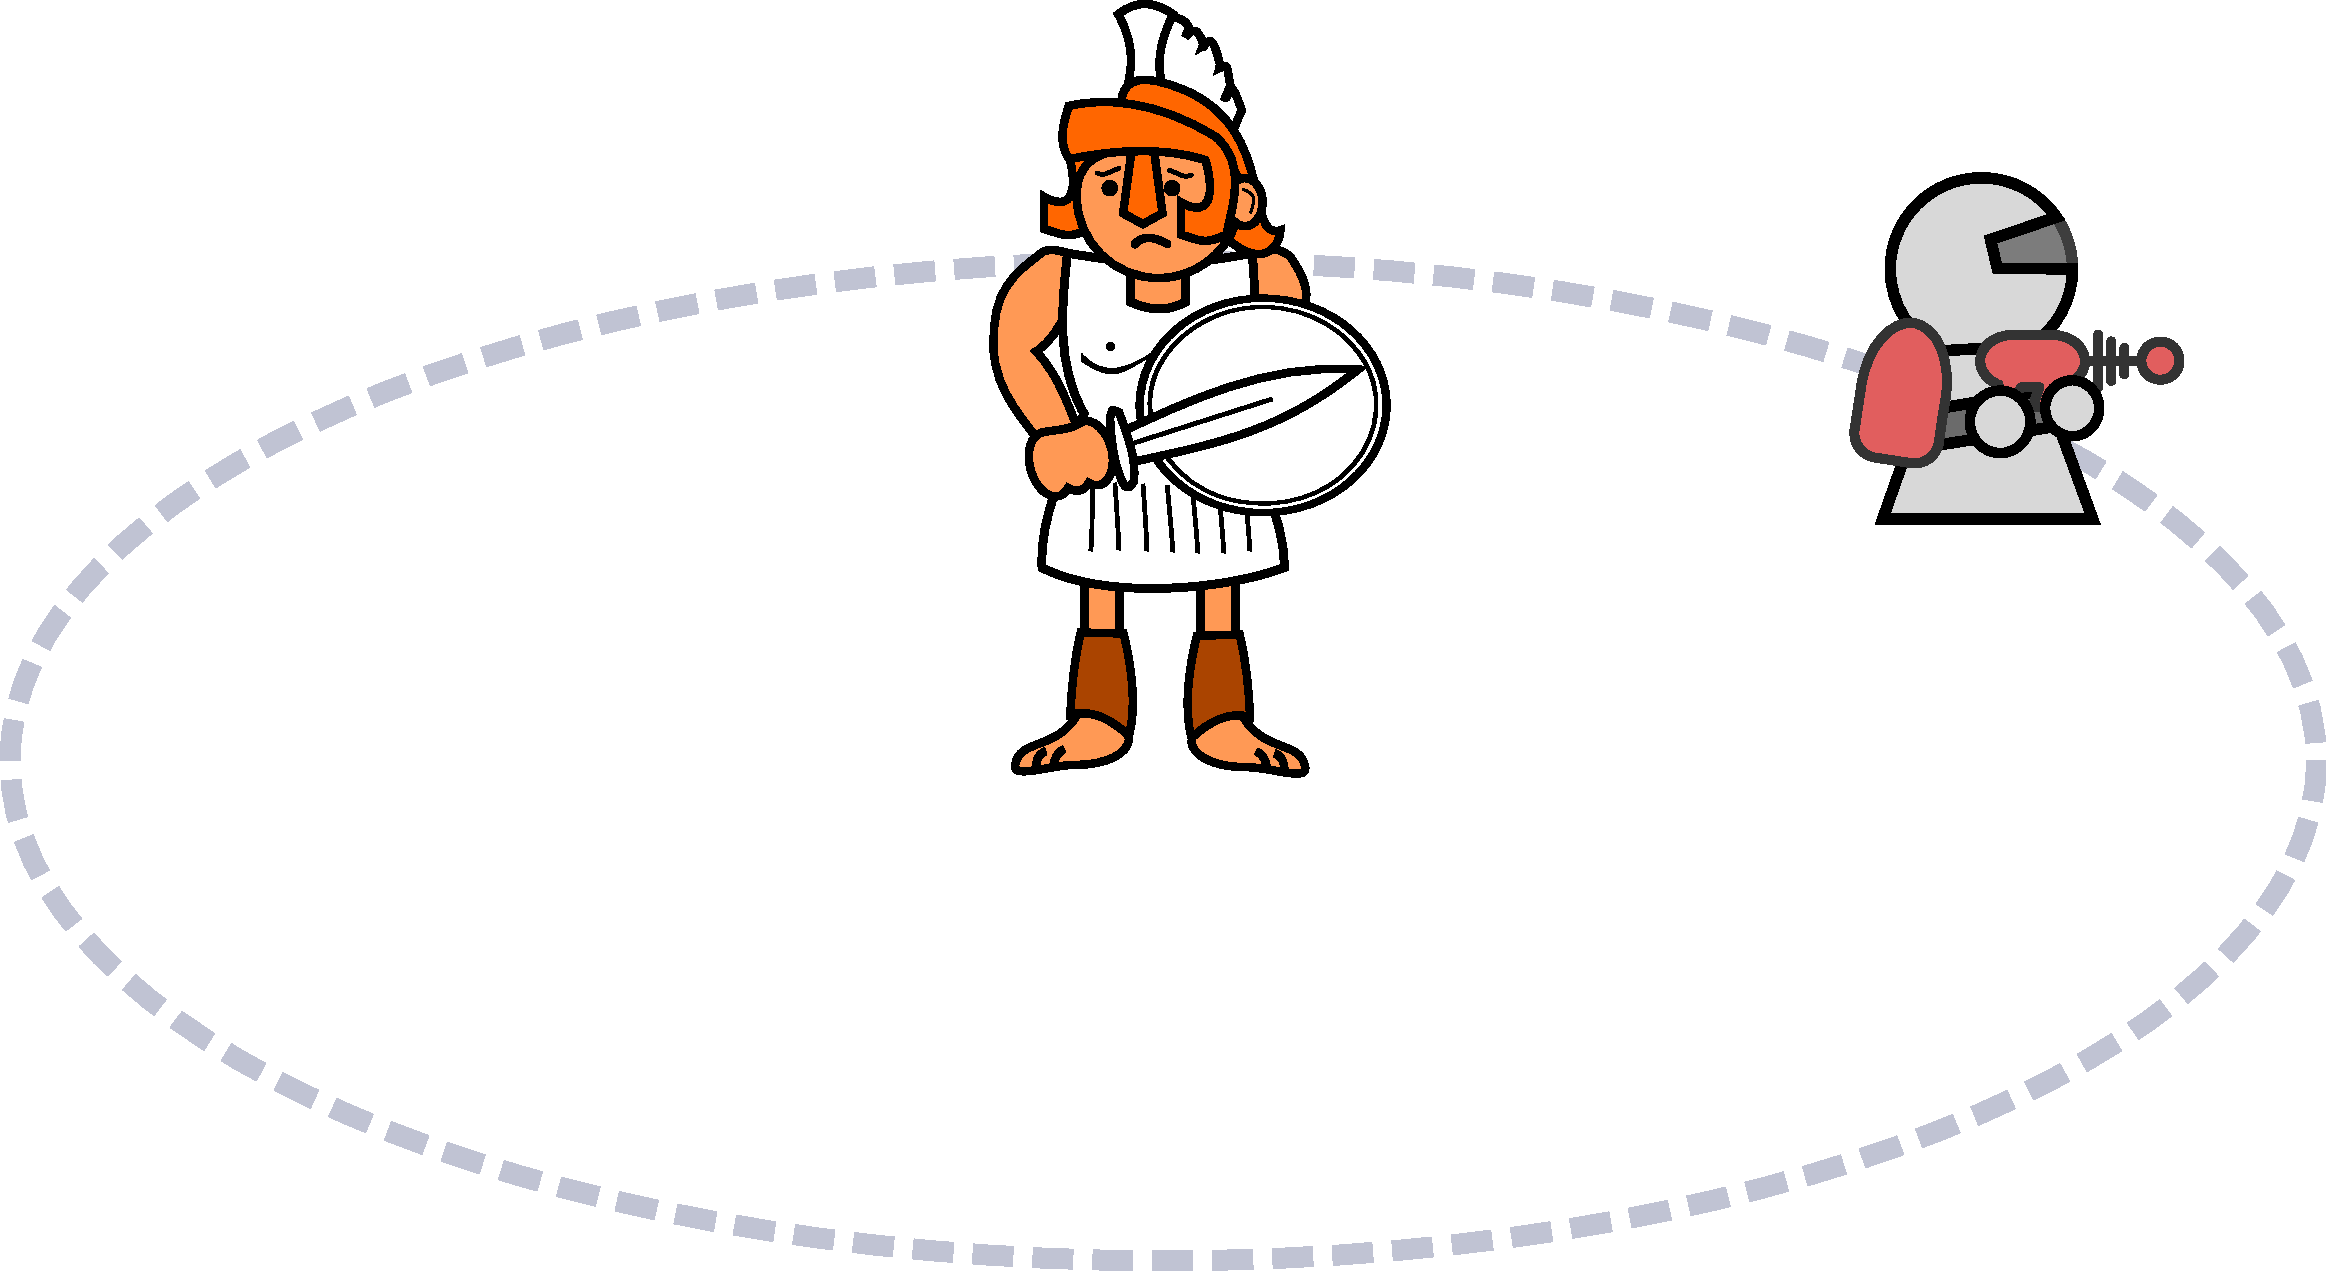
\includegraphics[width = 0.7\textwidth]{./figure/human_robot_interaction}
	\end{figure}
	
	\begin{itemize}
		\item cooperative observation
		\item assistance and protection
	\end{itemize}
	
\end{frame}

\begin{frame}{Neighboring function}{Human constraint}
	\begin{columns}
		\column{.6\linewidth}
		\begin{minipage}[c]{\linewidth}
			\begin{figure}
				\centering
				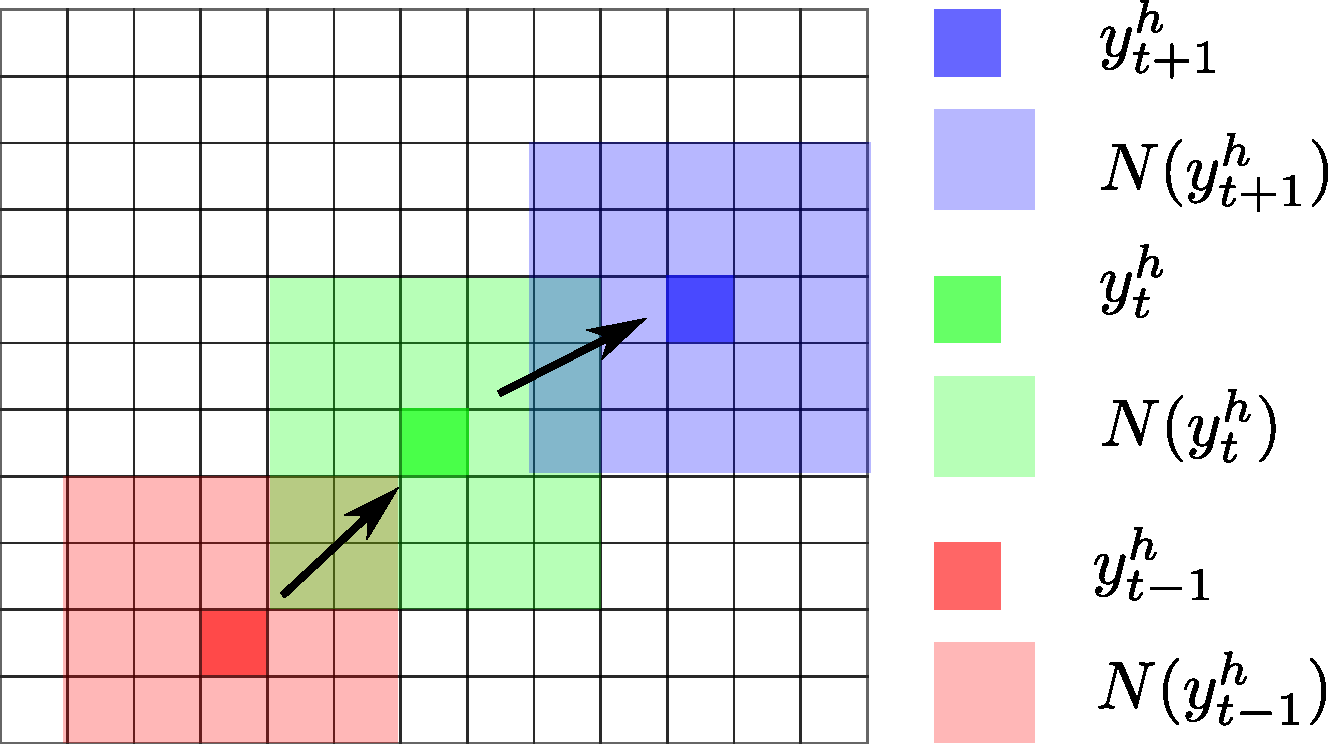
\includegraphics[width = \textwidth]{./figure/humanConstraint}
				%\caption{An example of human constraint.}
			\end{figure}
		\end{minipage}
		
		\column{.4\linewidth}
		\begin{minipage}[c]{\linewidth}
			\begin{itemize}
				\item { human path $ \{ y^{h}_{1} \cdots y^{h}_{T} \} $ }
				\item { neighboring function $ N( y^{h}_{t} ) $ }
			\end{itemize}
		\end{minipage}
	\end{columns}
	
\end{frame}

\begin{frame}{Related work}{ Using a greedy heuristic}
\begin{block}{C.~Chekuri 2005\cite{1530718}}
\begin{itemize}
\item Recursive greedy on a graph topoplogy
\item Edge cost $ \Rightarrow $ Budget 
\end{itemize}
\end{block}
\begin{block}{A.~Singh 2007\cite{singh2007efficient}}
\begin{itemize}
\item Spatial decomposition
\item Recursive greedy of multiple robots
\end{itemize}
\end{block}
\end{frame}

\begin{frame}{Related work}{Using a coarse-to-fine dynamic programming}
\begin{block}{C.~Raphael 2001\cite{Raphael2001}}
Coarse-to-fine backtracking
\end{block}
\begin{figure}
	\centering
	\includegraphics[width = 0.5\textwidth]{./figure/coarse_to_fine_DP}
\end{figure}
\end{frame}






\section{Human constraint}

\begin{frame}{Human constraint}{constraint}

\end{frame}

% All of the following is optional and typically not needed. 

\end{document}


